\documentclass{article}

\usepackage{float}
\usepackage{microtype}
\usepackage{indentfirst}
\usepackage{amsmath}
\usepackage{tikz}
\usepackage{graphicx}
\usetikzlibrary{arrows,automata}
\usepackage[utf8]{inputenc}
\usepackage[portuguese]{babel}

\title{Relatório 3 \- MIPS Multiciclo}
\author{%
    Mikael Luan da Silva Saraiva, \\
    João Vitor Maia Neves Cordeiro, \\
    Paola de Oliveira Abel
    }

\begin{document}
    \maketitle

    \section{Introdução}

    Neste projeto desenvolveremos um processador MIPS multiciclo, criando seus
    arquivos de descrição em VHDL e realizando as devidas simulações além de
    analisar seu funcionamento.

    \section{Descrição do Sistema}

    Eu preciso completar isso

    \section{Principais características}

    Contem um unidade de memoria, banco de registradores com 32 registradores,
    um a ULA, possui processamento multiciclo é mais rápido que o monociclo,
    pois pode realizar mais de uma etapa de um processo por ciclo de clock,
    desde que usem áreas diferentes. No projeto multiciclo consideramos que um
    ciclo de clock pode acomodar no máximo uma das seguintes operações: Um
    acesso a memoria, um acesso ao banco de registradores (duas leituras e uma
    escrita, ou uma operação da ULA). Consequentemente quaisquer dados
    produzidos por uma dessas três unidades funcionais precisam ser salvos em
    um registrador temporário para uso em um ciclo posterior, se eles não forem
    salvos poderia haver a possibilidade de uma disputa de sincronização,
    levando ao uso de um valor incorreto.

    \subsection{Circuitos}

    \begin{figure}[H]
        \centering % para centralizarmos a figura
        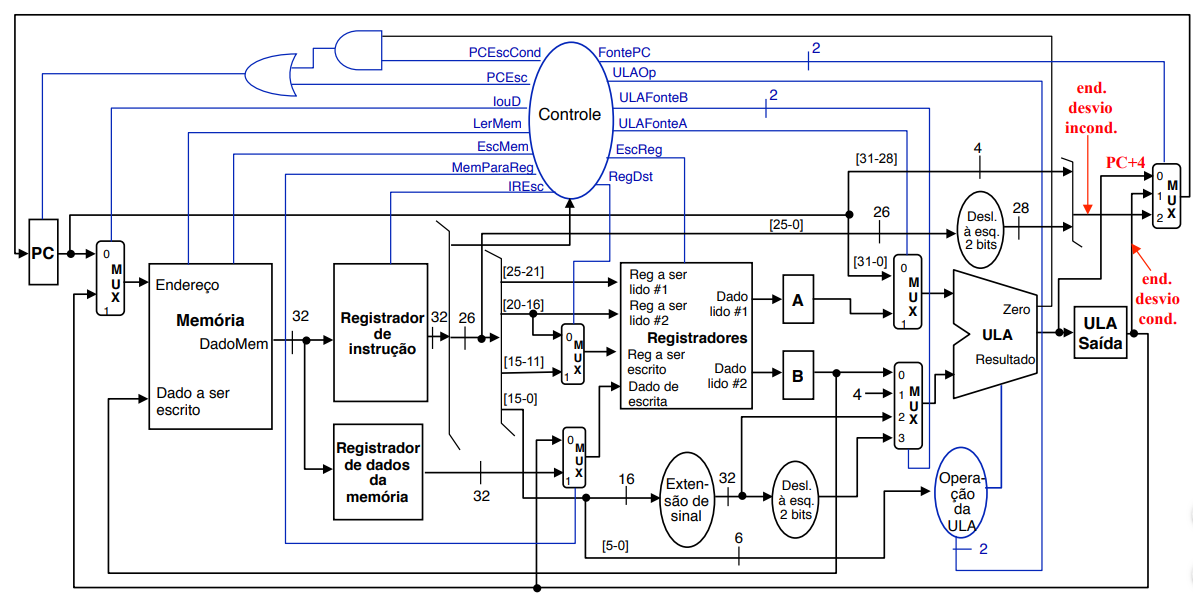
\includegraphics[width=\textwidth]{circuito_mips.png} % leia abaixo
        \label{figura:mips}
    \end{figure}

    \subsection{Diagramas}

    Eu preciso completar isso

    \subsection{Maquinas de Estado}

    \begin{figure}[H]
        \centering % para centralizarmos a figura
        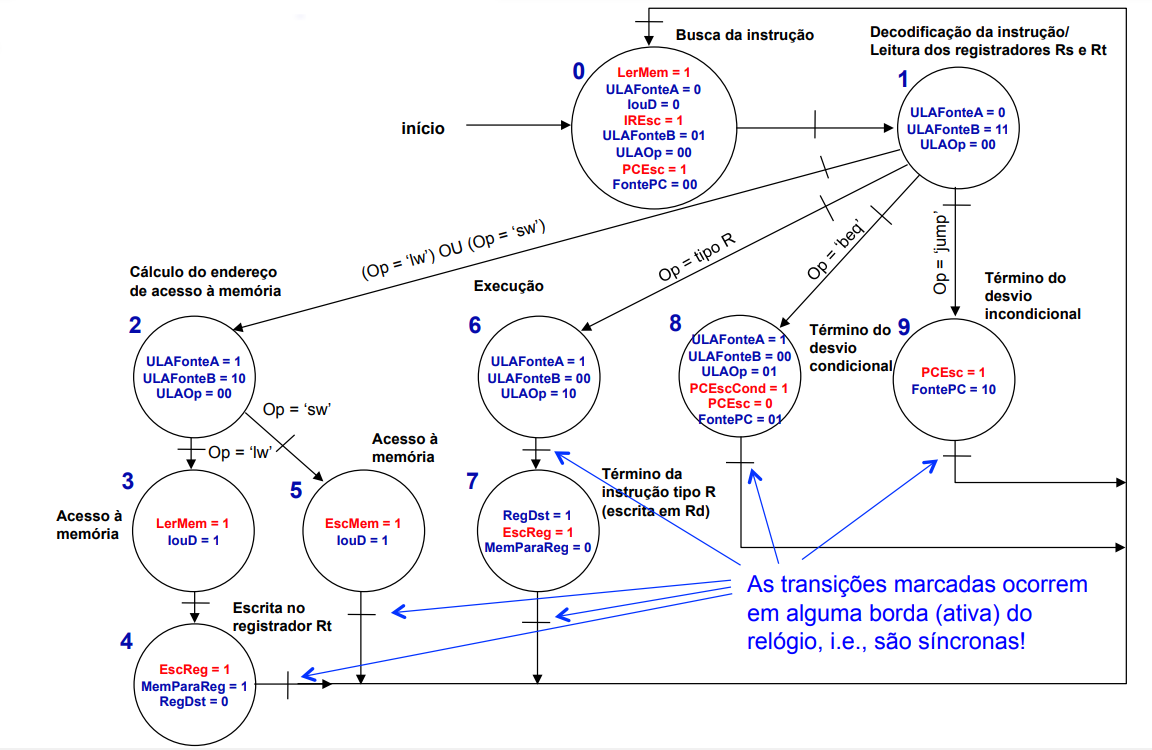
\includegraphics[scale=1.5]{maquina_estados.png} % leia abaixo
        \label{figura:maquina}
    \end{figure}

    \section{Resultados de atrasos}

    Eu preciso completar isso

    \section{Utilização da placa}

    Eu preciso completar isso

    \section{Discussão dos resultados}

    Eu preciso completar isso

    \section{Conclusões}

    Eu preciso completar isso

\end{document}
